\documentclass[../main.tex]{subfiles}
\begin{document}
\section{路径规划}

\subsection*{路径规划算法结构概览}
\begin{enumerate}
    \item \textbf{路径搜索算法}
    \begin{enumerate}
        \item 精确解法:
        \begin{itemize}
            \item \hyperref[subsubsec:BFS]{BFS算法}
            \item \hyperref[subsubsec:Dijkstra]{Dijkstra算法}
        \end{itemize}
        \item 近似算法:
        \begin{itemize}
            \item \hyperref[subsubsec:Astar]{A*算法}
            \item \hyperref[subsubsec:Ant]{蚁群算法}
        \end{itemize}
    \end{enumerate}

    \item \textbf{\hyperref[subsec:resolution_complete]{分辨率完备的连通图构建}}
    \begin{enumerate}
        \item \hyperref[item:res:roadmap]{行车图法}
        \item \hyperref[item:res:cell]{单元分解法}
        \item \hyperref[item:res:apf]{人工势场法}
    \end{enumerate}

    \item \textbf{\hyperref[subsec:probabilistic_complete]{概率完备的连通图构建}}
    \begin{enumerate}
        \item \hyperref[item:prob:prm]{PRM}
        \item \hyperref[item:prob:rrt]{RRT}
    \end{enumerate}

    \item \textbf{\hyperref[subsec:recent_research]{路径规划近期研究}}
\end{enumerate}



\subsection{导航规划及其组成}\label{subsec:navigation_planning}
\begin{enumerate}
    \item \textbf{导航规划的概念}:在给定环境的全局或局部知识以及一个或者一系列目标位置的条件下,使机器人能够根据知识和传感器感知信息高效可靠地到达目标位置。
    \item \textbf{导航规划的组成}:
    通常可以分解为3个问题,三者的关系:互补
    \begin{itemize}
        \item \textbf{路径规划}(战略方法):根据所给定的地图和目标位置,规划一条使机器人到达目标位置的路径。
        \item \textbf{避障规划}(战术方法):根据所得到的实时传感器测量信息,调整路径/轨迹以避免发生碰撞
        \item \textbf{轨迹规划}(机器人执行):根据机器人的运动学模型和约束,寻找适当的控制命令,将可行路径转化为可行轨迹
    \end{itemize}
\end{enumerate}

\subsection{路径规划的基本概念}\label{subsec:pathplanning_basic}
\begin{enumerate}
    \item \textbf{路径规划}:根据所给定的地图和目标位置,规划一条使机器人到达目标位置的路径。
    \\{\small\kaishu (只考虑工作空间的几何约束,不考虑机器人的运动学模型和约束可将移动机器人简化为工作空间中的一个点)}
    \item \textbf{工作空间与位形空间}:
    \begin{itemize}
        \item \textbf{工作空间}:移动机器人上的参考点能达到的空间集合,机器人采用位置和姿态描述,并需考虑体积。
        \item \textbf{位形空间}:机器人成为一个可移动点,不考虑姿态、体积和非完整运动学约束,包括:
            \begin{itemize}
                \item \textbf{障碍物空间}:不可行的位形集合。{\small\kaishu (在该空间中,机器人会与障碍物发生碰撞)}
                \item \textbf{障碍物空间}:可行的位形集合。{\small\kaishu (在该空间中,机器人将无碰地安全移动。路径规划就是在自由位形空间中为机器人寻找一条路径,使其从初始位置运行到目标位置)}
            \end{itemize}
    \end{itemize}
    \begin{figure}[H]
        \centering
        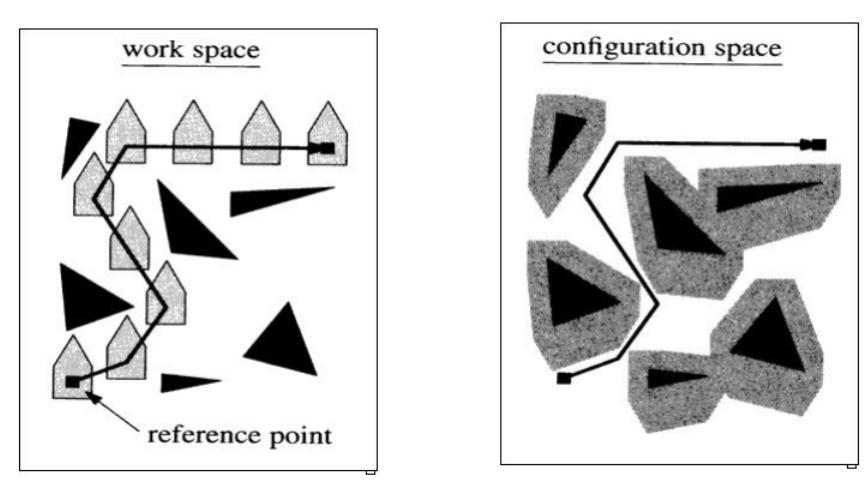
\includegraphics[width=0.6\textwidth]{images/1.png}
        \caption{工作空间(左)VS 位形空间(右)}
    \end{figure}
    \item \textbf{算法}:
        \begin{itemize}
            \item \textbf{完备性的概念}:当解存在时,能够在有限的时间内找到解。
            \item \textbf{挑战}:在连续空间内搜索,难以保证时间。
        \end{itemize}
    \item \textbf{路径规划的两个基本问题}:拓扑连通图、最优路径搜索
    \item \textbf{拓扑连通图构建方法:}
    \begin{itemize}
        \item \textbf{基本思路}:对空间作离散化
        \item {两种完备}:
            \begin{itemize}
                \item \textbf{分辨率完备}:解析性离散化,确保获得可行解。
                \\{\small\kaishu (典型算法:行车图法、单元分解法、势场法)}
                \item \textbf{概率完备}:随机采样离散化,基于概率,使得获得解的概率趋近于1。
                \\{\small\kaishu (典型算法:PRM、RRT)}
            \end{itemize}
    \end{itemize}
\end{enumerate}

\subsection{路径搜索算法}\label{subsec:path_search}
\begin{enumerate}
    \item \textbf{最优路径搜索算法}:在构建形成的连通图中搜索最优路径:
        \begin{itemize}
            \item \textbf{精确解法}:生成精确最优解,遍历获得所有路径后选择最优解
                \begin{itemize}
                    \item \textbf{典型方法}:深度优先法、广度优先法→优先级定义的广度优先法、Dijstra算法;
                    \item \textbf{问题}:耗时,难以满足快速规划要求
                \end{itemize}
            \item \textbf{近似算法}:不会遍历所有路径
                \begin{itemize}
                    \item \textbf{典型方法}:
                        \begin{itemize}
                            \item 启发式搜索算法:A*、D*、Focused D*
                            \item 准启发式搜索算法:退火、进化、蚁群
                        \end{itemize}
                \end{itemize}
        \end{itemize}

    \item \textbf{精确解法:广度优先算法(BFS)}\label{subsubsec:BFS}
    
        \begin{figure}[H]
            \centering
            \begin{subfigure}[b]{0.32\textwidth}
                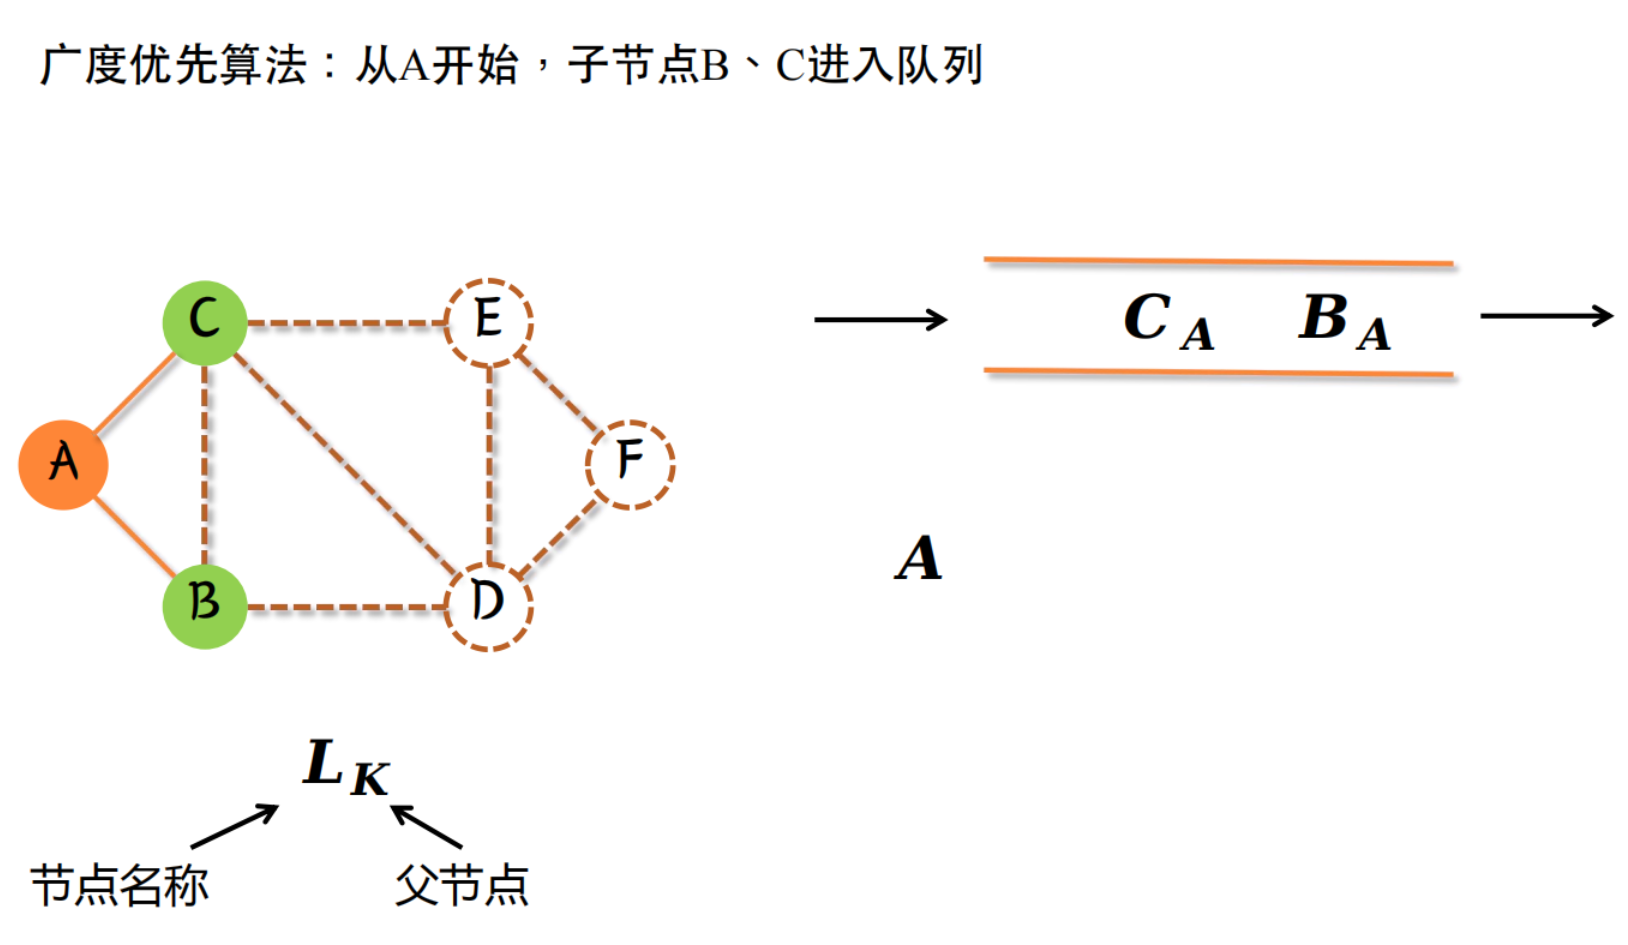
\includegraphics[width=\textwidth]{images/BFS/1.png}
            \end{subfigure}
            \begin{subfigure}[b]{0.32\textwidth}
                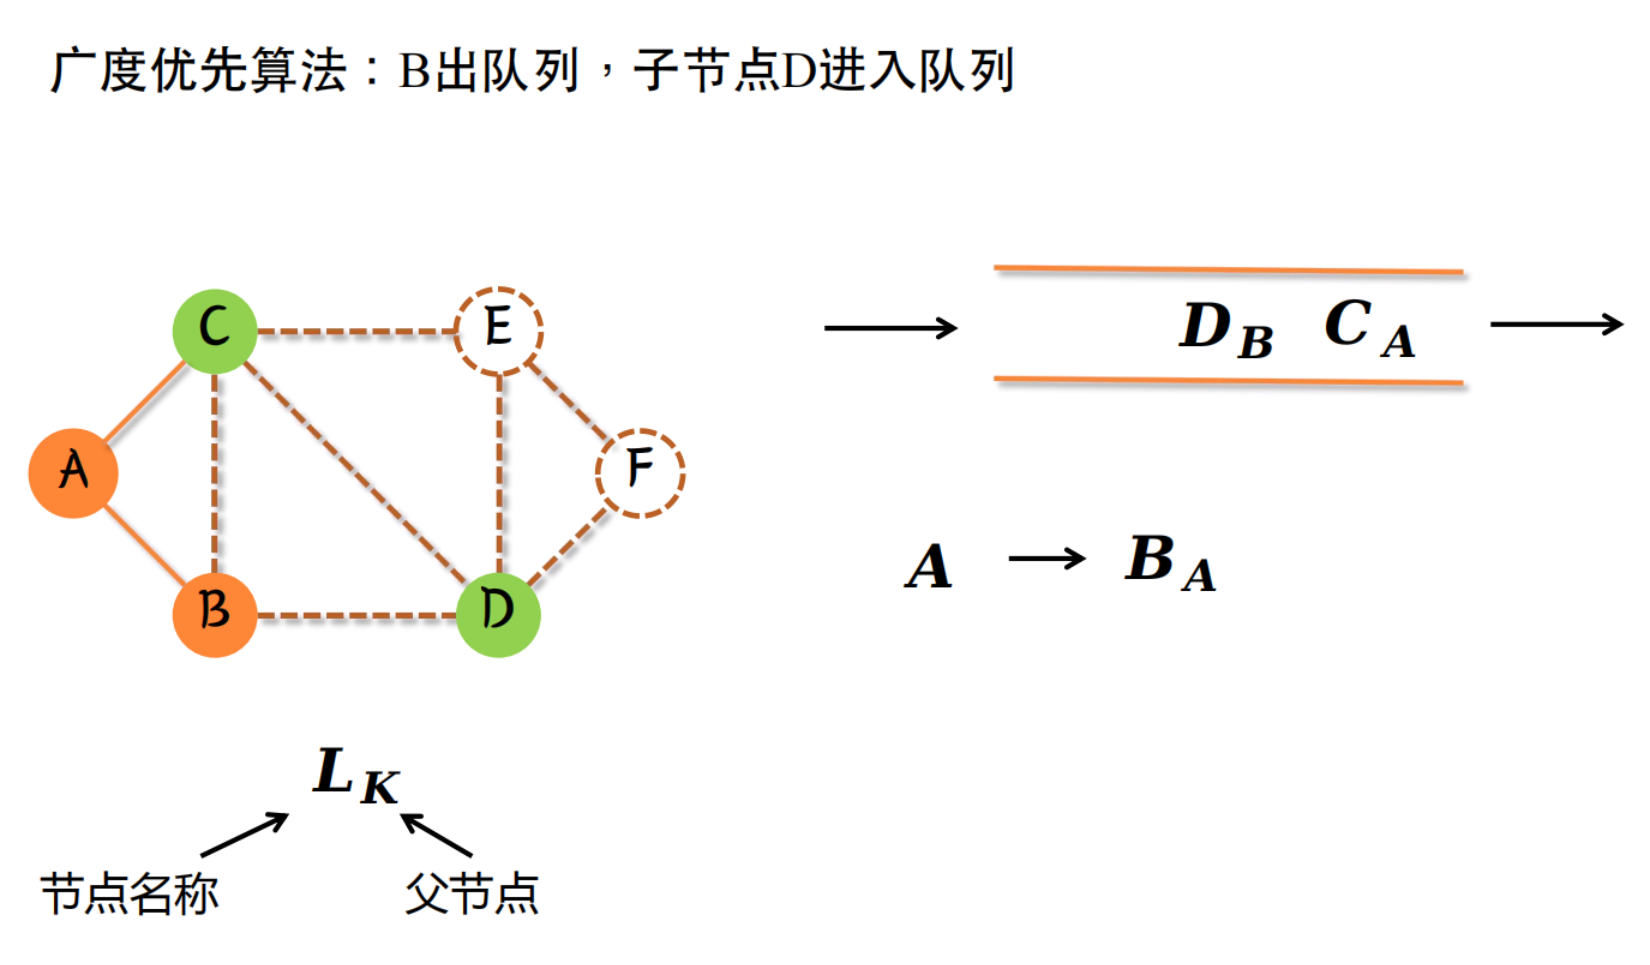
\includegraphics[width=\textwidth]{images/BFS/2.png}
            \end{subfigure}
            \begin{subfigure}[b]{0.32\textwidth}
                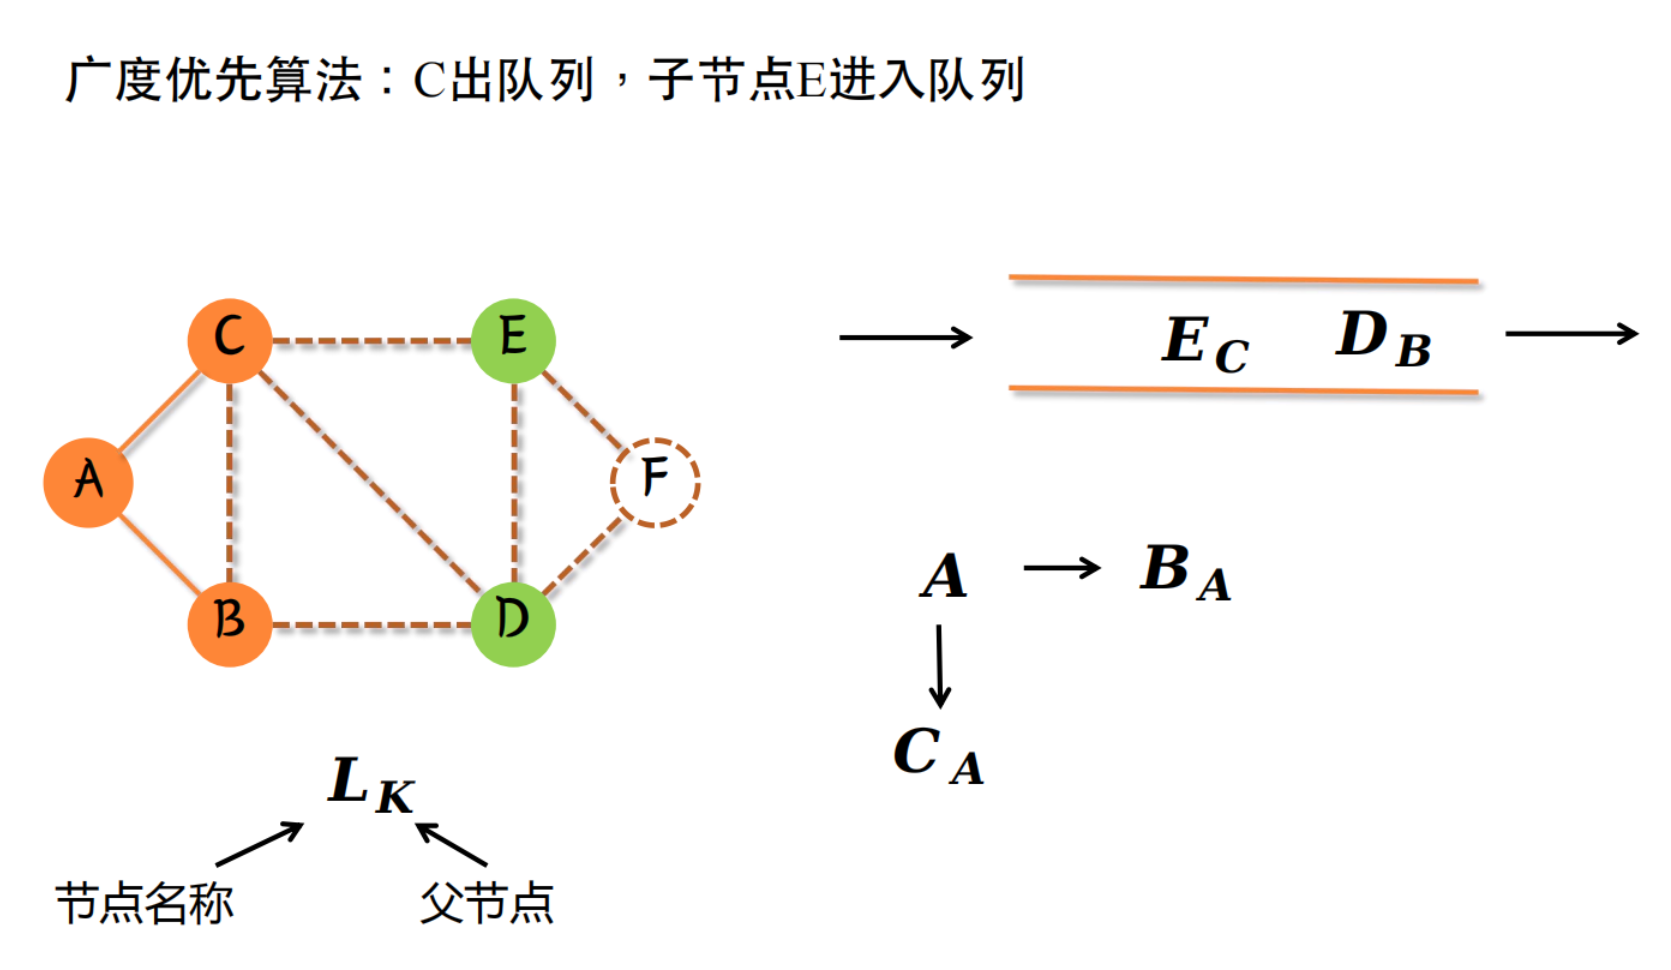
\includegraphics[width=\textwidth]{images/BFS/3.png}
            \end{subfigure}
            \vspace{0.5em}
            \begin{subfigure}[b]{0.32\textwidth}
                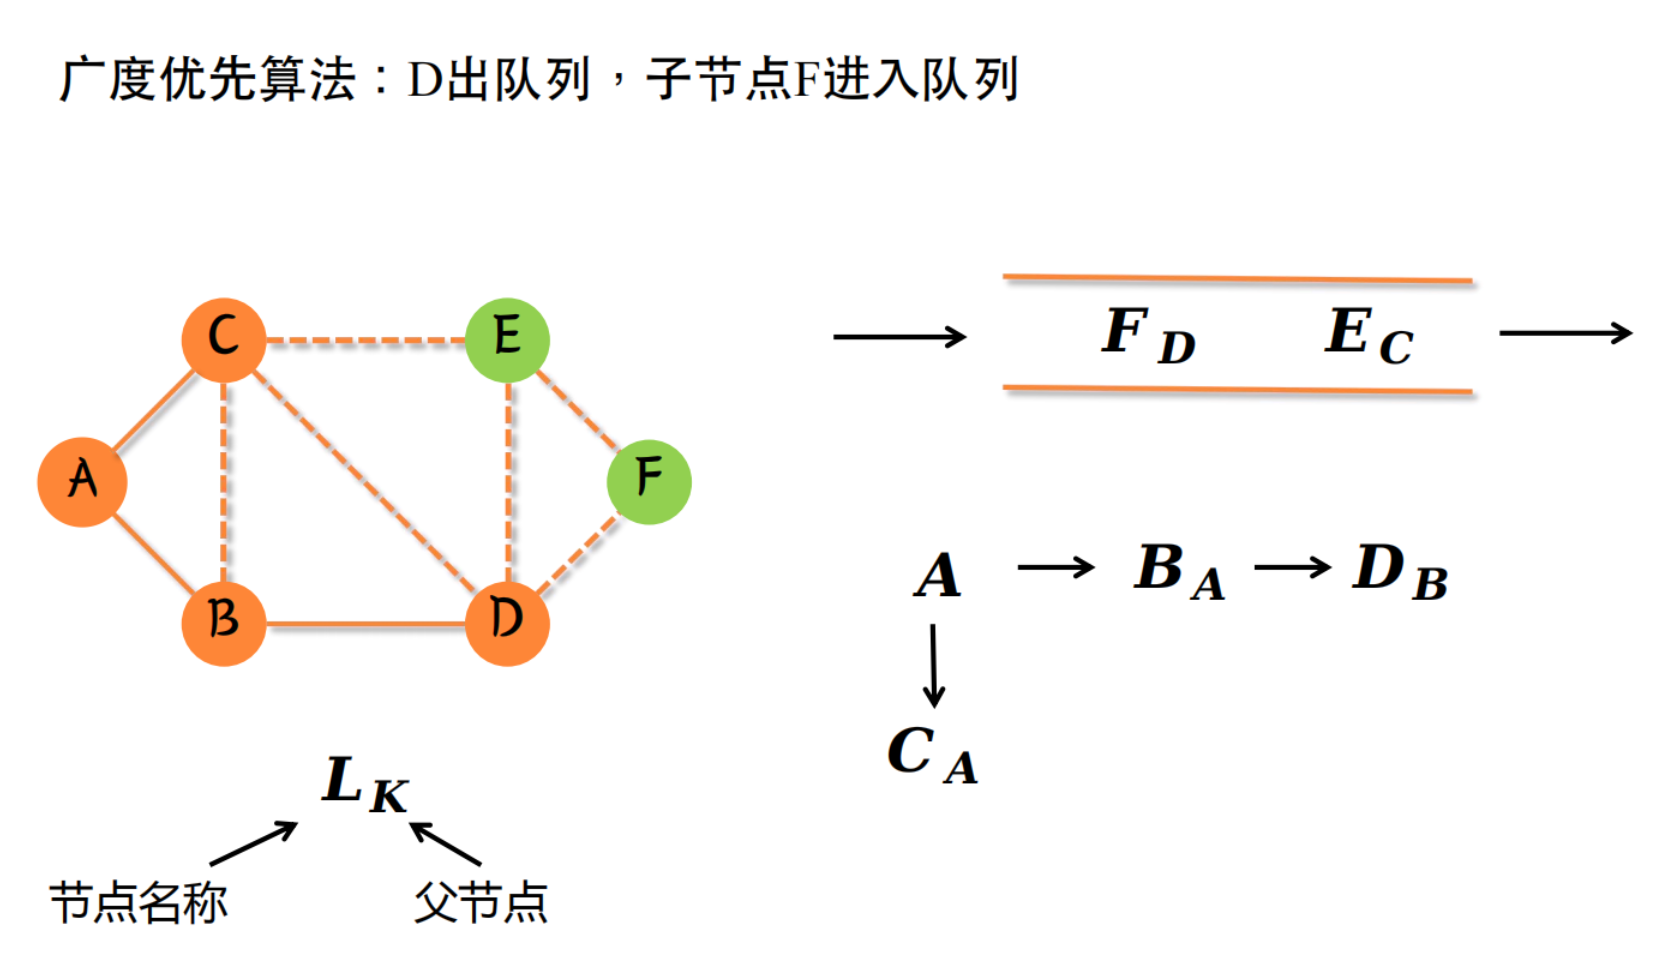
\includegraphics[width=\textwidth]{images/BFS/4.png}
            \end{subfigure}
            \begin{subfigure}[b]{0.32\textwidth}
                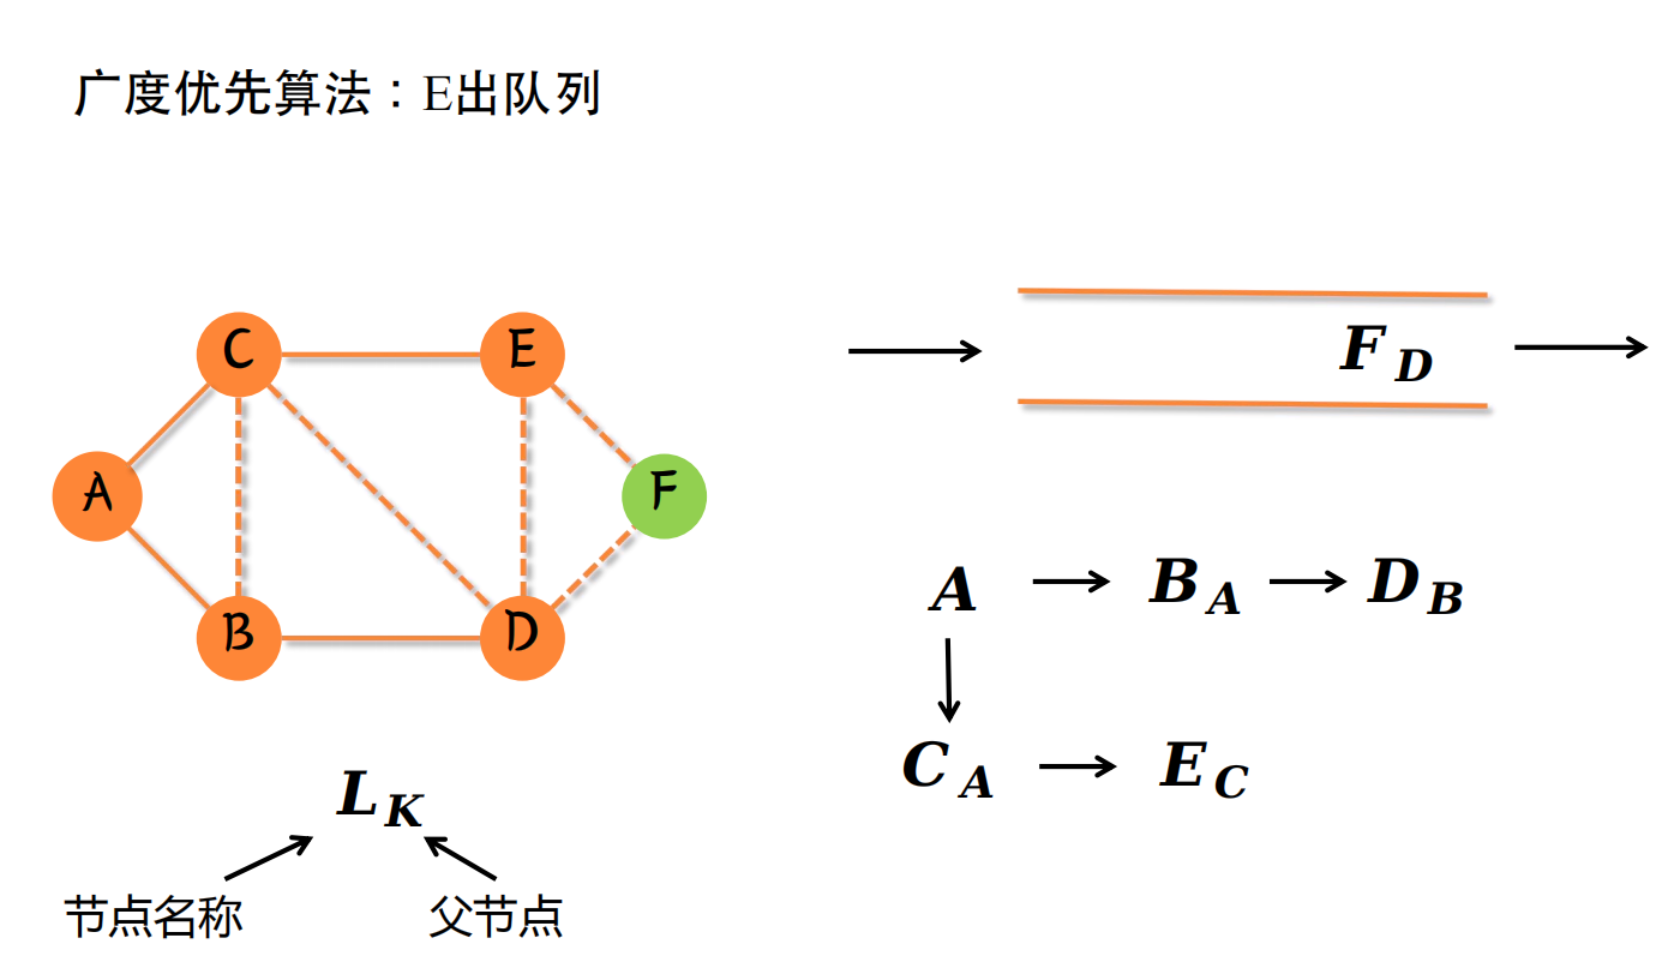
\includegraphics[width=\textwidth]{images/BFS/5.png}
            \end{subfigure}
            \begin{subfigure}[b]{0.32\textwidth}
                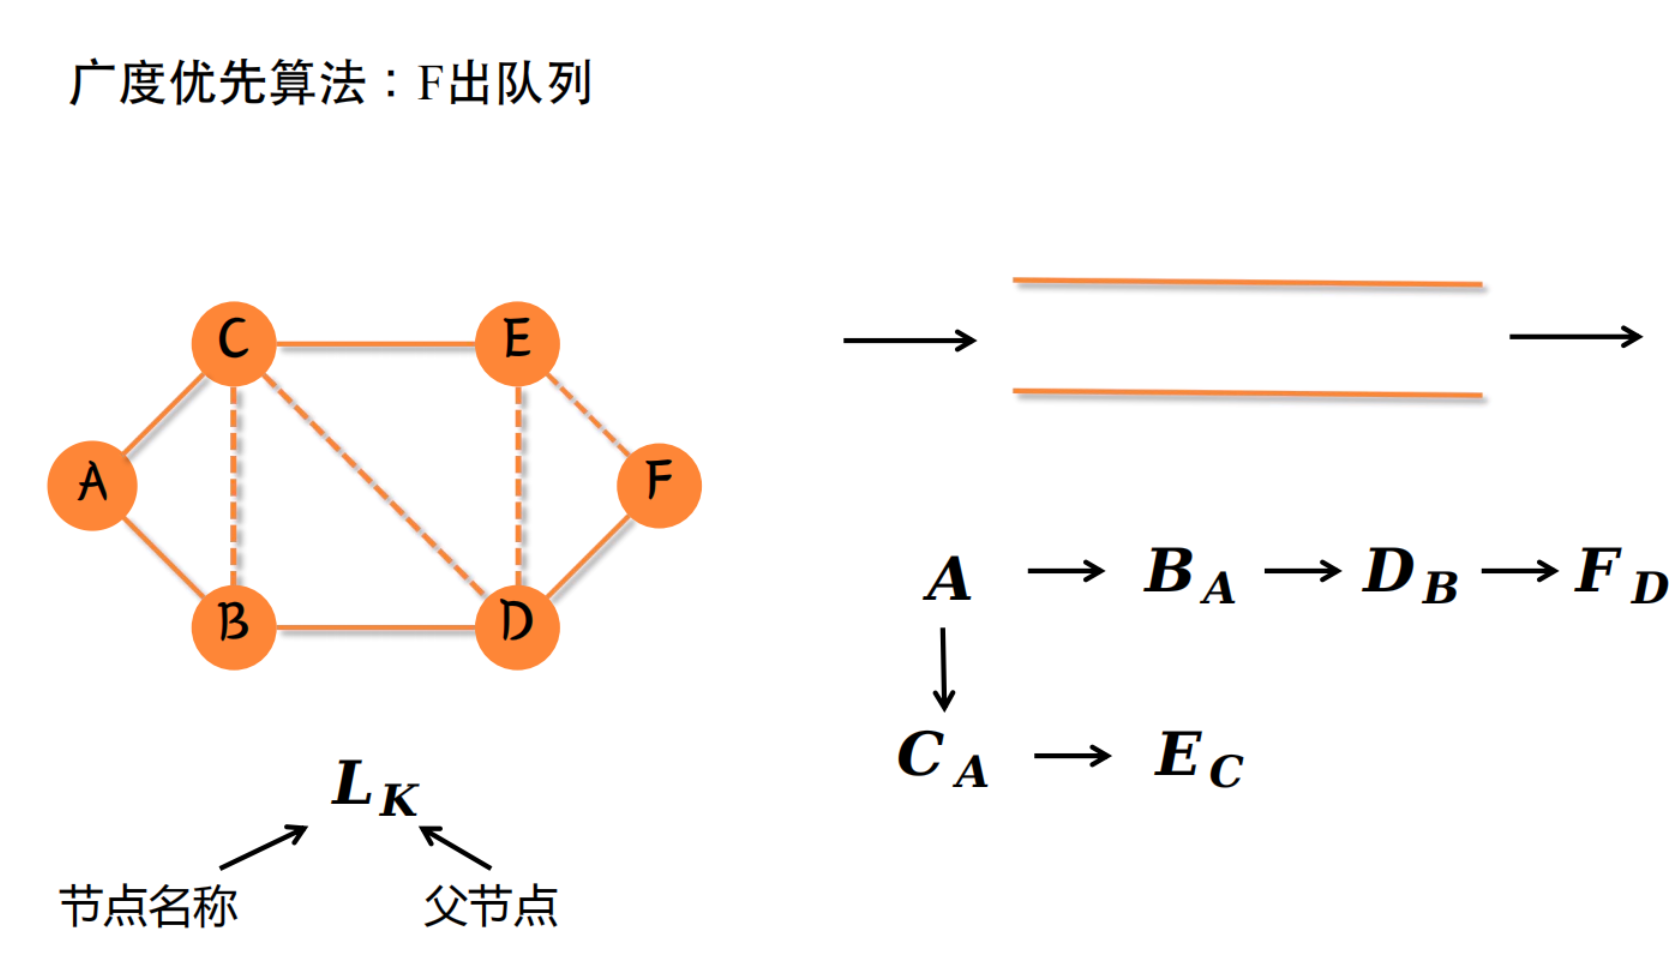
\includegraphics[width=\textwidth]{images/BFS/6.png}
            \end{subfigure}
            \caption{BFS算法流程}
        \end{figure}
        
    \item \textbf{精确解法:DIJKSTRA算法}\label{subsubsec:Dijkstra}
        \begin{itemize}
            \item \textbf{思想}:优先级定义的广度优先搜索
            \item \textbf{流程}:在有向图中以起始点为中心按\textbf{路径长度}递增方式层层向外扩展,直到扩展到终止点。
                \begin{itemize}
                    \item {\small\kaishu 设置两个集合S和T, S存放已经找到最短路径的顶点,T是尚未确定路径的顶点集合,同时也描述了起始点经过集合S中顶点到该点的最短路径及长度。}
                    \item {\small\kaishu 每次更新时,从T中找出路径最短的点加入到集合S,T中顶点最短路径及长度则根据加入点作为中间点后起始点到该点距离是否减小来决定是否更新。}
                \end{itemize}
                \begin{figure}[H]
                    \centering
                    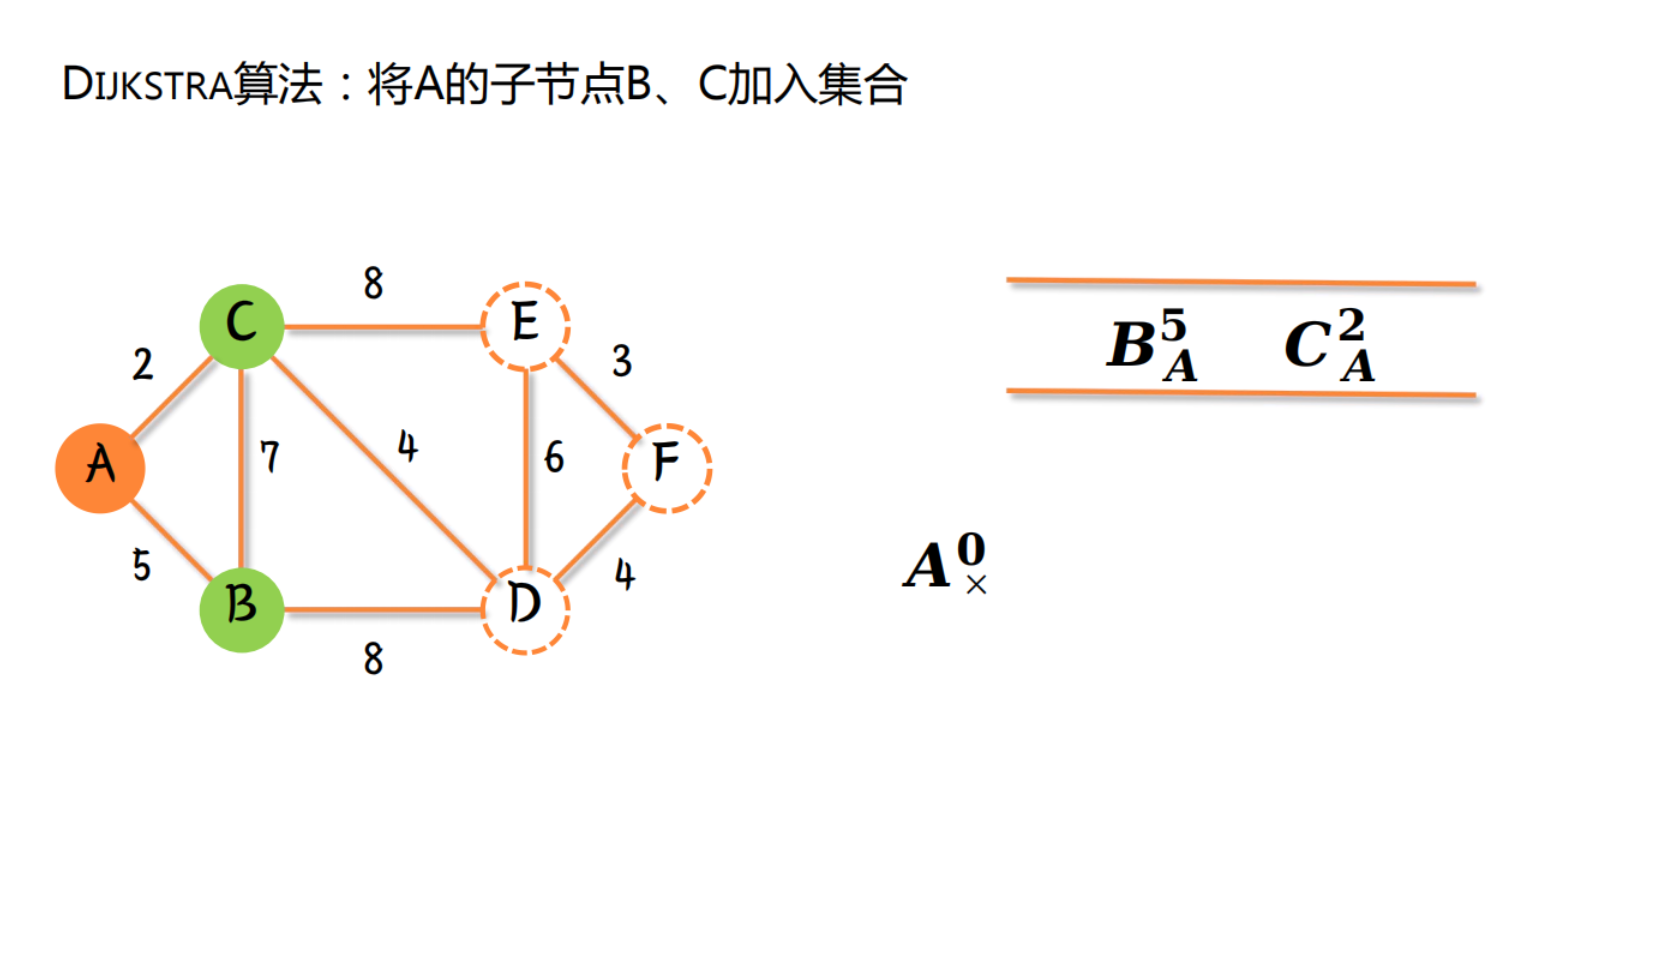
\includegraphics[width=0.9\textwidth]{images/DIJKSTRA/1.png}
                    \caption{dijkstra算法流程}
                \end{figure}
        \end{itemize}
    
    \item \textbf{近似算法:A*(启发式搜索算法)}\label{subsubsec:Astar}
    \begin{itemize}
        \item \textbf{思想}:优先级定义的广度优先搜索。
        \item \textbf{流程}:根据启发式评估函数在连通图中寻找最优路径。\footnote{A*算法在Dijkstra算法的基础上引入启发式函数$h(n)$,使得节点扩展更具有倾向性和目的性而不是漫无目的地四处扩展,通过$f(n)=g(n)+h(n)$综合考虑已走路径代价与估计代价,从而更高效地找到最优路径。一个比较好的动画示例是https://www.redblobgames.com/pathfinding/a-star/introduction.html}              
        \\ {\small\kaishu 当选择下一个探索结点时,通过启发式评价函数进行评估,选择路径代价最小的结点作为下一步探索结点而跳转其上。}
            \begin{itemize}
                \item 评价函数定义为:
                \[
                f(n) = g(n) + h(n)
                \]
                其中:
                \begin{itemize}
                    \item \( n \):表示结点;
                    \item \( g(n) \):表示从起始点到结点 \( n \) 的实际代价;
                    \item \( h(n) \):为从结点 \( n \) 到目标点的最佳路径估计代价。
                \end{itemize}
            \end{itemize}
        \item \textbf{路径成本的计算($h(n)$的选取)}:欧氏距离或曼哈顿距离,当$h(n)$可采纳时最优。
        \begin{figure}[H]
            \centering
            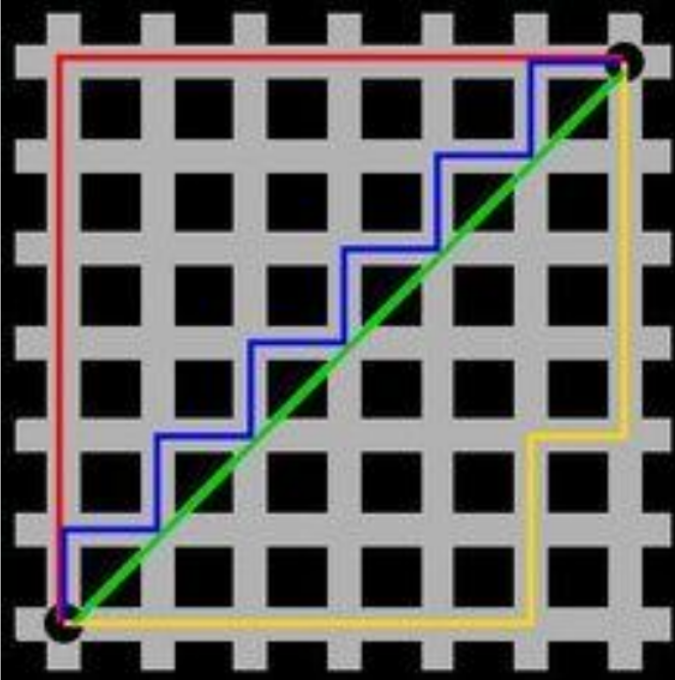
\includegraphics[width=0.3\textwidth]{images/hn.png}
            \caption{曼哈顿距离(红)VS 欧氏距离(绿)VS 等价曼哈顿距离(黄、蓝)}
        \end{figure}
    \end{itemize}

    \item \textbf{近似算法:蚁群算法(准启发式搜索算法)}\label{subsubsec:Ant}
        \begin{itemize}
            \item \textbf{思想}:一个蚂蚁的行走路径表示待优化问题的一个可行解。
            \item \textbf{流程}:根据概率函数选择路径并通过信息素更新逐步收敛。
            \item \textbf{特点}:
                \begin{itemize}
                    \item 优点:可适应动态环境,可并行;
                    \item 缺点:计算量大、参数敏感。
                \end{itemize}
        \end{itemize}
\end{enumerate}

\textbf{小结:路径搜索算法}
\begin{table}[H]
    \centering
    \small
    \begin{tabular}{cccccc}
        \toprule
        \textbf{算法} & \textbf{完备性} & \textbf{最优性} & \textbf{$a$} & \textbf{$b$} & \textbf{说明}\\
        \midrule
        BFS & 1 & 1 & 1 & 0 & 无启发,按层搜索\\
        DFS & 0 & 0 & 1 & 0 & 无启发,按深搜索\\
        Dijkstra & 1 & 1 & 1 & 0 & 仅考虑实际代价$g(n)$\\
        A*算法 & 1 & 1$^\ast$ & 1 & 1 & 综合代价与启发式:$f=ag+bh$\\
        贪心算法 & 0 & 0 & 0 & 1 & 仅考虑启发函数$h(n)$\\
        可调贪婪算法 & 0$\sim$1 & 0$\sim$1 & $a\in[0,1)$ & $b\in(0,1]$ & 权重可调,折中策略\\
        \bottomrule
    \end{tabular}
        \caption{基于$f = a g + b h$的路径搜索算法比较($^\ast$ 当$h(n)$可采纳时最优)}
    \label{tab:astar_compare_cn}
\end{table}

\subsection{分辨率完备的连通图构建}\label{subsec:resolution_complete}
\begin{enumerate}
    \item \textbf{行车图法}\label{item:res:roadmap}
        \begin{figure}[H]
            \centering
            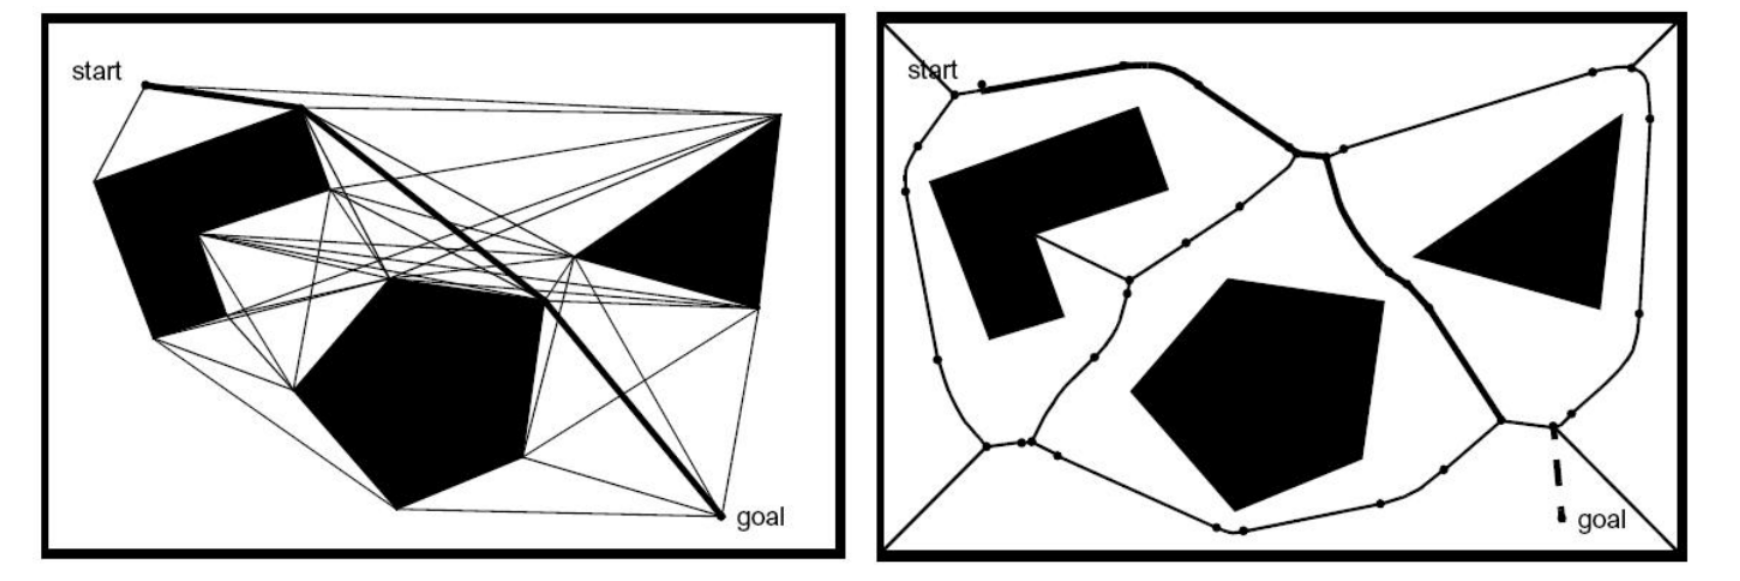
\includegraphics[width=0.6\textwidth]{images/xingchetu.png}
            \caption{Visibility graph(左)VS Voronoi diagram(右)}
        \end{figure}
        \textbf{基本思想:}基于障碍物几何形状分解位形空间,将自由空间的连通性用一维曲线的网格表示,在加入起始点和目标点后,在该一维无向连通图中寻找一条无碰路径。
        \begin{enumerate}
            \item \textbf{可视图法}\label{item:res:visibility}
                \begin{itemize}
                    \item \textbf{组成}:所有连接可见\footnote{可见:指顶点之间无障碍物}顶点对的边\footnote{初始位置和目标位置也作为顶点}。
                    \item \textbf{优点}:
                        \begin{itemize}
                            \item 非常简单(尤其是环境地图用多边形描述物体时)
                            \item 可得到在路径长度上最优的解
                        \end{itemize}
                    \item \textbf{缺点}:
                        \begin{itemize}
                            \item 所得路径过于靠近障碍物,不够安全
                        \end{itemize}
                    \item \textbf{解决办法}:
                        \begin{itemize}
                            \item 膨胀:以远大于机器人半径的尺寸膨胀障碍物,但容易造成可行路径的消失
                            \item 距离:在路径规划后修改所得路径,使其与障碍物保持一定的距离
                        \end{itemize}
                \end{itemize}
            \item \textbf{Voronoi diagram}\label{item:res:voronoi}
                \begin{itemize}
                    \item \textbf{基本思想}:取障碍物之间的中间点,以最大化机器人和障碍物之间的距离
                    \item \textbf{构建方法}:
                        \begin{enumerate}
                            \item 自由空间内每一点计算到最近障碍物距离
                            \item 在垂直于二维空间平面的轴上表示到该点障碍物距离(类似画直方图)
                            \item 当某个点到两/多个障碍物距离相等时,其距离点处出现尖峰
                            \item 连接尖峰点得到边
                        \end{enumerate}
                    \item \textbf{优点}:
                        \begin{itemize}
                            \item 安全
                        \end{itemize}
                    \item \textbf{缺点}:
                        \begin{itemize}
                            \item 计算:复杂
                            \item 路径长度:比可视图法更长
                            \item 适用性:不适用于短距离定位传感器
                        \end{itemize}
                    \item \textbf{解决办法}:
                        \begin{itemize}
                            \item 膨胀:以远大于机器人半径的尺寸膨胀障碍物,但容易造成可行路径的消失
                            \item 距离:在路径规划后修改所得路径,使其与障碍物保持一定的距离
                        \end{itemize}
                \end{itemize}
        \end{enumerate}
    \item \textbf{单元分解法}\label{item:res:cell}
        \begin{figure}[H]
            \centering
            \begin{subfigure}[b]{0.48\textwidth}
                \centering
                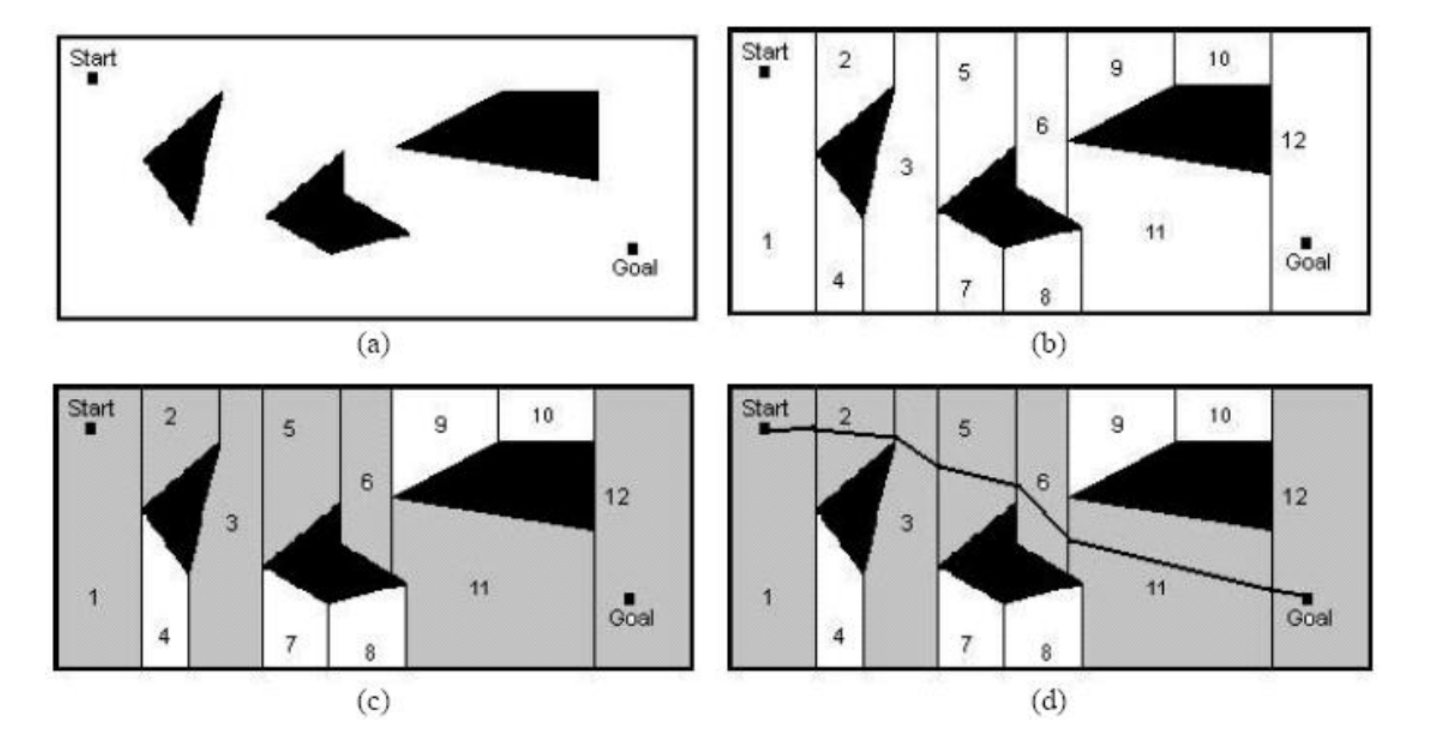
\includegraphics[width=\linewidth]{images/jingquedanyuanfenjie.png}
                \caption{精确单元分解示意图}
                \label{fig:exact-cell}
            \end{subfigure}
            \hfill
            \begin{subfigure}[b]{0.48\textwidth}
                \centering
                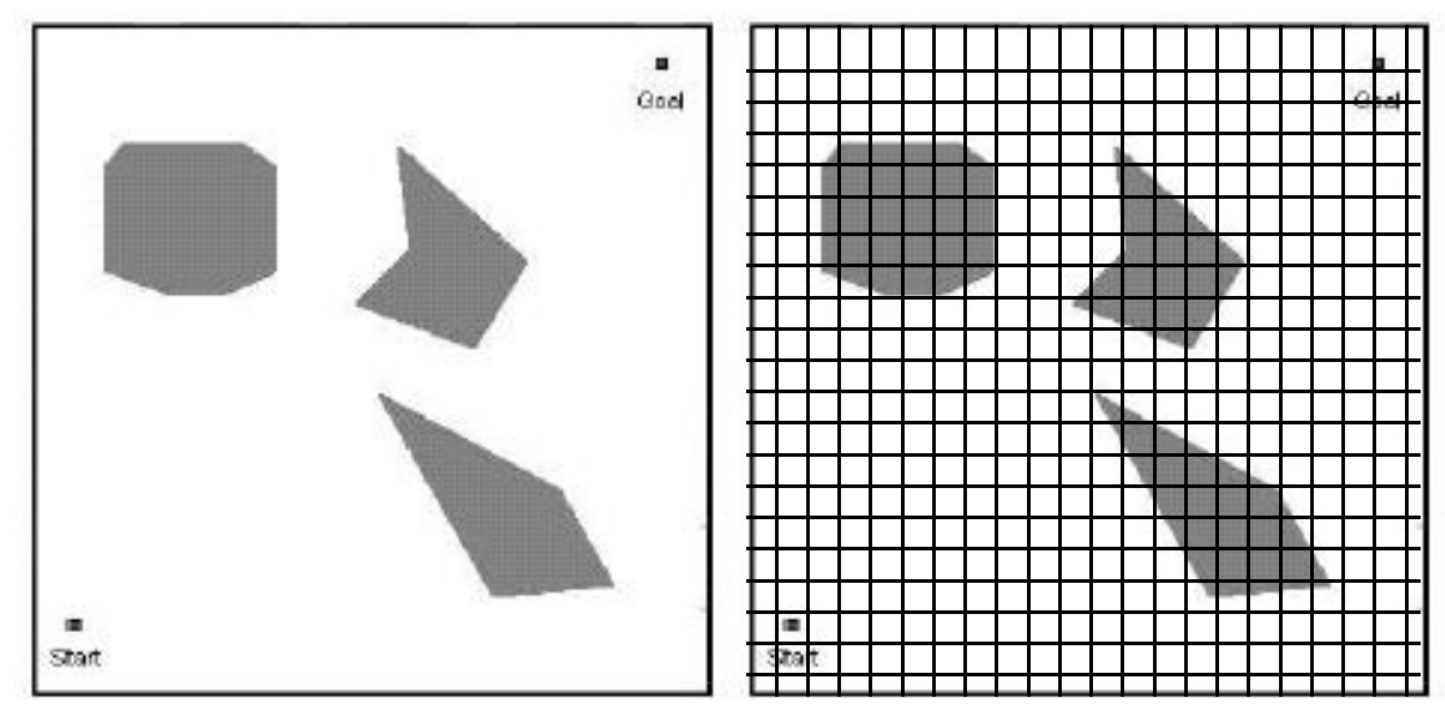
\includegraphics[width=\linewidth]{images/shangebiaoshifa.png}
                \caption{近似单元分解示意图}
                \label{fig:approx-cell}
            \end{subfigure}
        \end{figure}
    \textbf{基本思想}:
        \begin{enumerate}
            \item 将位形空间中的自由空间分为若干的小区域,每一个区域作为一个单元
            \item 以单元为顶点、以单元之间的相邻关系为边,构成一张连通图
            \item 在连通图中寻找包含初始姿态和目标姿态的单元,搜索连接初始单元和目标单元的路径
            \item 根据所得路径的单元序列生成单元内部的路径
        \end{enumerate}
      \textbf{主要方法}:精确单元分解和近似单元分解。
        \begin{enumerate}
            \item \textbf{精确单元分解}\label{item:res:cell:exact}
                \begin{itemize}
                    \item \textbf{基本思想}:边界严格基于环境形状几何分解,所得单元完全空闲
                    \item \textbf{优点}:
                        \begin{itemize}
                            \item 机器人不需要考虑它在每个空闲单元中的具体位置,只需要考虑如何从一个单元移动到相邻的空闲单元
                            \item 单元数与环境大小无关
                        \end{itemize}
                    \item \textbf{缺点}:
                        \begin{itemize}
                            \item 计算:计算效率极大地依赖于环境中物体的复杂度
                        \end{itemize}
                \end{itemize}            
            \item \textbf{近似单元分解}\label{item:res:cell:approx}
                \begin{itemize}
                    \item \textbf{基本思想}:并不是每个单元都是完全被占或者完全空闲的,因此分解后的单元集合是对实际地图的一种近似
                    \item \textbf{典型方法}:栅格表示法——将环境分解成若干个大小相同的栅格。
                    \item \textbf{优点}:
                        \begin{itemize}
                            \item 机器人不需要考虑它在每个空闲单元中的具体位置,只需要考虑如何从一个单元移动到相邻的空闲单元
                            \item 单元数与环境大小无关
                        \end{itemize}
                    \item \textbf{缺点}:
                        \begin{itemize}
                            \item 计算:计算效率极大地依赖于环境中物体的复杂度
                        \end{itemize}
                \end{itemize}      
            \item \textbf{可变大小的近似单元分解}\label{item:res:cell:var}
                \begin{itemize}
                    \item \textbf{典型方法}:四叉树表示法——递归地把环境分为4个大小相等的子区域,直到每个区域中所包含的基本元素全为0或全为1。
                \end{itemize}
            \begin{figure}[H]
                \centering
                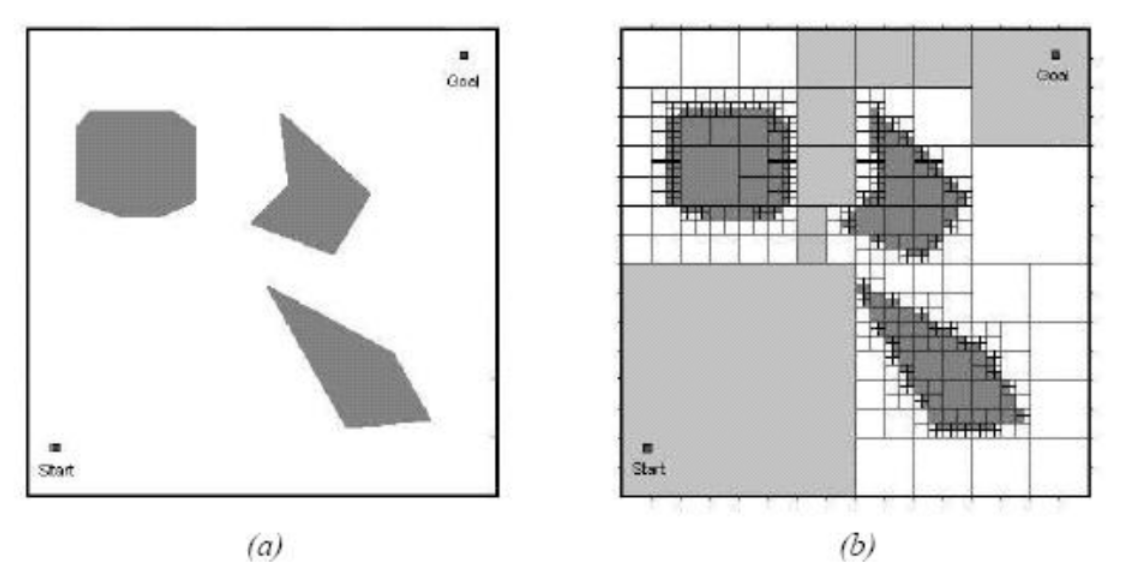
\includegraphics[width=0.6\textwidth]{images/kebiandaxiao.png}
                \caption{可变大小的近似单元分解四叉树表示法}
            \end{figure}
        \end{enumerate}
    \item \textbf{人工势场法}\label{item:res:apf}
            \begin{figure}[H]
                \centering
                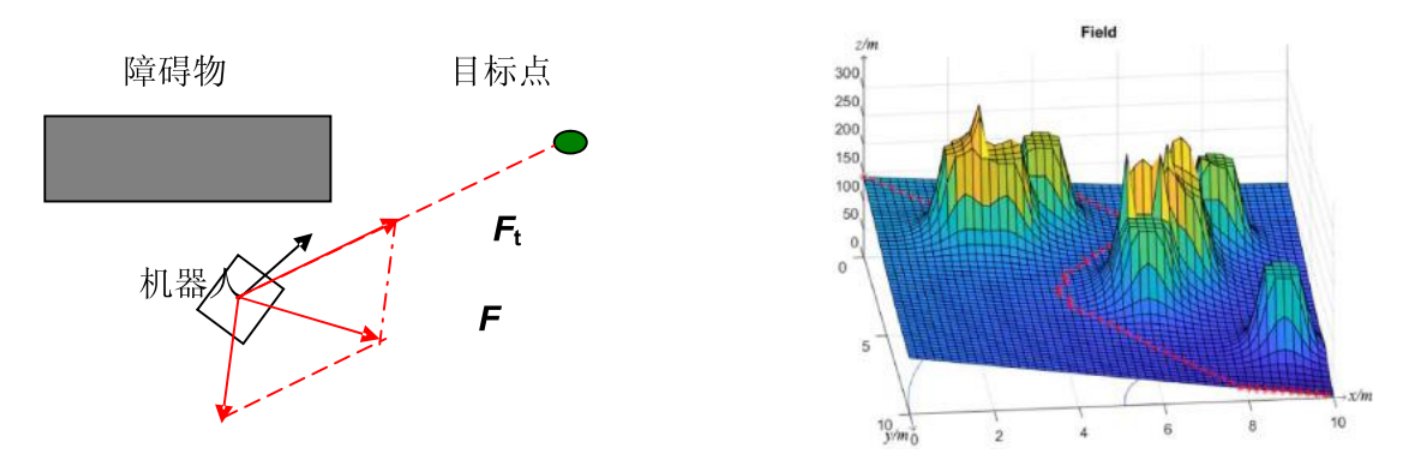
\includegraphics[width=0.6\textwidth]{images/rengongshichang.png}
                \caption{人工势场法示意图}
            \end{figure}
        \begin{itemize}
            \item \textbf{基本思想}:目标点对机器人产生吸引力,障碍物对机器人产生排斥力——所有力的合成构成机器人的控制律。
            \item \textbf{构建步骤}:
                \begin{enumerate}
                    \item \textbf{构建人工势场}(吸引 + 排斥)
                    \begin{itemize}
                        \item \textit{目标的吸引势}:
                        \[
                        U_{\mathrm{att}}(\mathbf{x})=
                        \begin{cases}
                            K_a\,\lVert \mathbf{x}-\mathbf{x}_d\rVert^2, & \lVert \mathbf{x}-\mathbf{x}_d\rVert \le d_a,\\[4pt]
                            K_a\!\left(2d_a\,\lVert \mathbf{x}-\mathbf{x}_d\rVert - d_a^2\right), & \lVert \mathbf{x}-\mathbf{x}_d\rVert > d_a,
                        \end{cases}
                        \]
                        \textit{其中 \(K_a\) 为系数,\(\mathbf{x}\) 为被评估点,\(\mathbf{x}_d\) 为目标点,\(d_a\) 为距离阈值。}
                        \item \textit{障碍的排斥势}(以最近障碍表面点距离 \(\rho(\mathbf{x})\) 与作用半径 \(\rho_0\)):
                        \[
                        U_{\mathrm{rep}}(\mathbf{x})=
                        \begin{cases}
                            \tfrac{1}{2}K_r\!\left(\dfrac{1}{\rho(\mathbf{x})}-\dfrac{1}{\rho_0}\right)^{\!2}, & \rho(\mathbf{x}) \le \rho_0,\\[8pt]
                            0, & \rho(\mathbf{x}) > \rho_0,
                        \end{cases}
                        \]
                        \textit{其中 \(K_r\) 为排斥系数}。
                    \end{itemize}
                
                    \item \textbf{根据势场计算力}(负梯度)
                    \[
                    \mathbf{F}_{\mathrm{att}}(\mathbf{x}) = -\nabla U_{\mathrm{att}}(\mathbf{x}) =
                    \begin{cases}
                        -2K_a(\mathbf{x}-\mathbf{x}_d), & \lVert \mathbf{x}-\mathbf{x}_d\rVert \le d_a,\\[6pt]
                        -2K_a d_a \dfrac{\mathbf{x}-\mathbf{x}_d}{\lVert \mathbf{x}-\mathbf{x}_d\rVert}, & \lVert \mathbf{x}-\mathbf{x}_d\rVert > d_a,
                    \end{cases}
                    \]
                    \[
                    \mathbf{F}_{\mathrm{rep}}(\mathbf{x}) = -\nabla U_{\mathrm{rep}}(\mathbf{x}) =
                    \begin{cases}
                        K_r\!\left(\dfrac{1}{\rho}-\dfrac{1}{\rho_0}\right)\!\dfrac{1}{\rho^{2}}\,\dfrac{\partial \rho}{\partial \mathbf{x}}, & \rho \le \rho_0,\\[10pt]
                        \mathbf{0}, & \rho > \rho_0,
                    \end{cases}
                    \]
                    其中
                    \[
                    \dfrac{\partial \rho}{\partial \mathbf{x}}
                    =\begin{pmatrix}\dfrac{\partial \rho}{\partial x}\\[2pt]\dfrac{\partial \rho}{\partial y}\end{pmatrix}
                    = \dfrac{\mathbf{x}-\mathbf{x}_0}{\rho},\qquad
                    \mathbf{x}_0 \text{ 为最近障碍表面点坐标。}
                    \]
                
                    \item \textbf{计算合力并生成控制律}
                    \[
                    \mathbf{F}(\mathbf{x}) = -\nabla U(\mathbf{x}) 
                    = \mathbf{F}_{\mathrm{att}}(\mathbf{x}) + \mathbf{F}_{\mathrm{rep}}(\mathbf{x}),
                    \]
                    将合力映射为控制输入(示例):
                    \[
                    \dot{\mathbf{x}} = k\,\mathbf{F}(\mathbf{x}) 
                    \quad \text{或} \quad 
                    \mathbf{a} = \frac{1}{m}\,\mathbf{F}(\mathbf{x}),
                    \]
                    方向即运动方向,大小可对应速度/加速度控制。
                \end{enumerate}

            \item \textbf{优点}:
                \begin{itemize}
                    \item 机器人是受人工势场影响的一个点,沿着势场方向就可以避开障碍物达到目标点
                    \item 不仅是一种路径规划方法,所构建的势场也构成了机器人的控制律,能够较好地适应目标的变化和环境中的动态障碍物,可以作为实时避障算法
                \end{itemize}
            \item \textbf{缺点}:
                \begin{itemize}
                    \item 存在局部最小,容易产生振荡和死锁\footnote{势场法仅用推斥势来表示障碍物,从而丢失了局部障碍物分布的详细信息}。(解决:见\hyperref[xiangliang]{向量势直方图法})
                \end{itemize}
        \end{itemize}

    
\end{enumerate}

\subsection{概率完备的连通图构建}\label{subsec:probabilistic_complete}
\begin{enumerate}
    \item \textbf{PRM}\label{item:prob:prm}
    \begin{figure}[H]
        \centering
        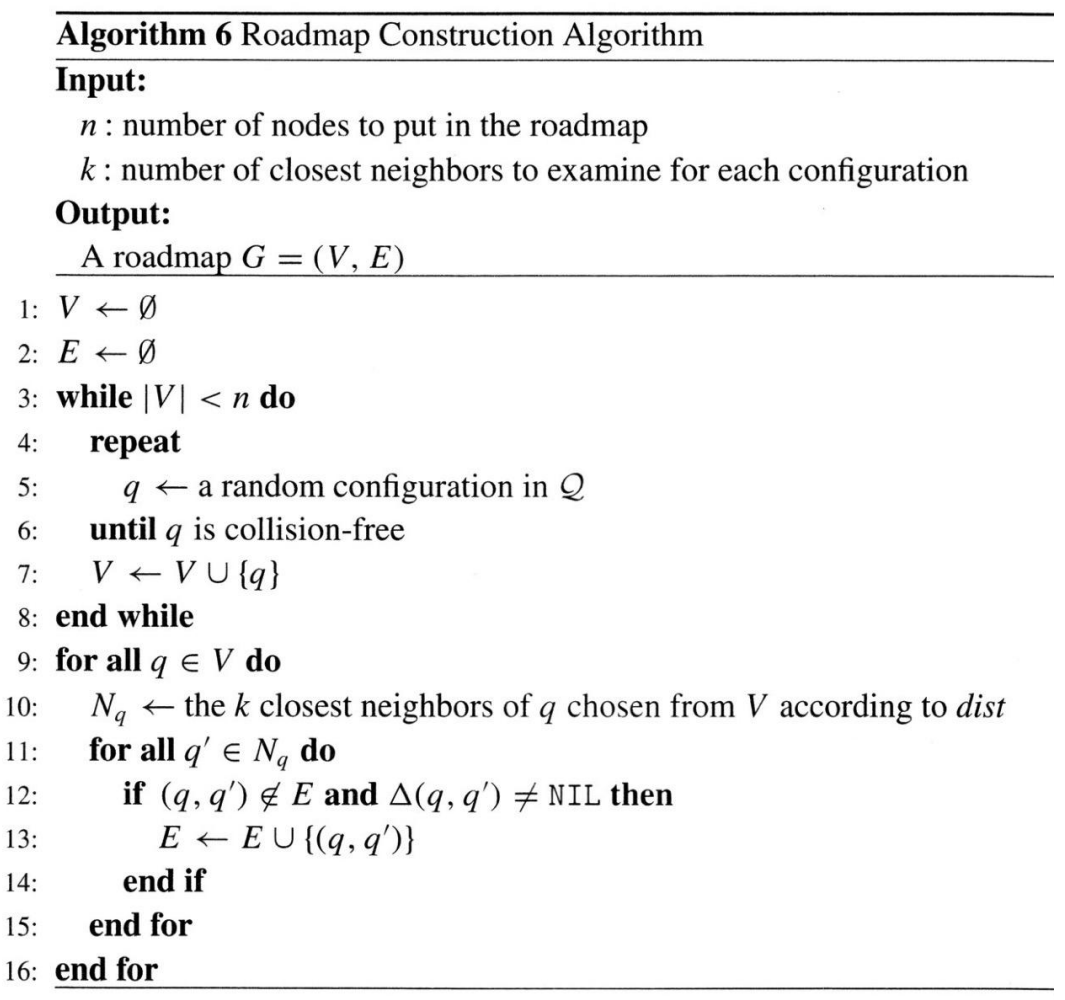
\includegraphics[width=0.6\textwidth]{images/prm.png}
        \caption{PRM算法流程}
    \end{figure}
    \textbf{基本步骤}:
        \begin{enumerate}
            \item 在整个位形空间坐标系中随机取点
            \item 对采样的姿态进行碰撞检测,无碰撞姿态成为图节点
            \item 每个图节点和其最近相邻的k个节点直线连接,保留无碰路径为图的边
            \item 边构成构成自由位形空间中的Roadmap
        \end{enumerate}
    \textbf{问题与解决方案}:   
        \begin{table}[H]
            \centering
            \small
            \begin{threeparttable}
            \begin{tabular}{@{}p{3cm}p{10cm}@{}}
                \toprule
                \textbf{问题} & \textbf{对应解决方式} \\
                \midrule
                随机位形选择 & 通常采用均匀随机采样方式 \\
                寻找最近邻点 & 可以采用KD树方法加速 \\
                生成局部路径 & 在一定范围内直接连接图节点 \\
                检查路径无碰 & 可以增量式取点或者二分法取点,判断点是否在障碍物区域内 \\
                ※非全联通情况 &
                采用困难度\tnote{1}作为该节点被选择为扩张节点的概率;选择后从该节点出发随机选择方向运动,若碰到障碍物则重新随机选,直到成功建立与其他单元连接。\\
                \bottomrule
            \end{tabular}
            \caption{PRM算法需要考虑的问题即对应解决方式}
            \label{tab:prm_considerations}
            \begin{tablenotes}
                \footnotesize
                \item[1] 对节点进行困难度表示,例如在该节点一定距离范围内的节点数的倒数、该节点到不与该节点连通的最近连通单元距离倒数、局部路径规划失败率等。
            \end{tablenotes}
            \end{threeparttable}
        \end{table}


        \textbf{优点}:
            \begin{itemize}
                \item 简化了对环境的解析计算,可以快速构建得到行车图
                \item 适用于高维度自由位形空间中的规划
                \item 是一个近似完备的路径规划方法
            \end{itemize}
        \textbf{缺点}:
            \begin{itemize}
                \item 连通性:对自由空间连通性表达的完整性依赖于采样次数
                \item 通用性:从算法通用性上来讲难以评估需要多少时间做充分采样
                \item 可行性:不考虑机器人执行的可行性
            \end{itemize}
    \item \textbf{RRT}\label{item:prob:rrt}
        \begin{figure}[H]
            \centering
            \begin{subfigure}[b]{0.45\textwidth}
                \centering
                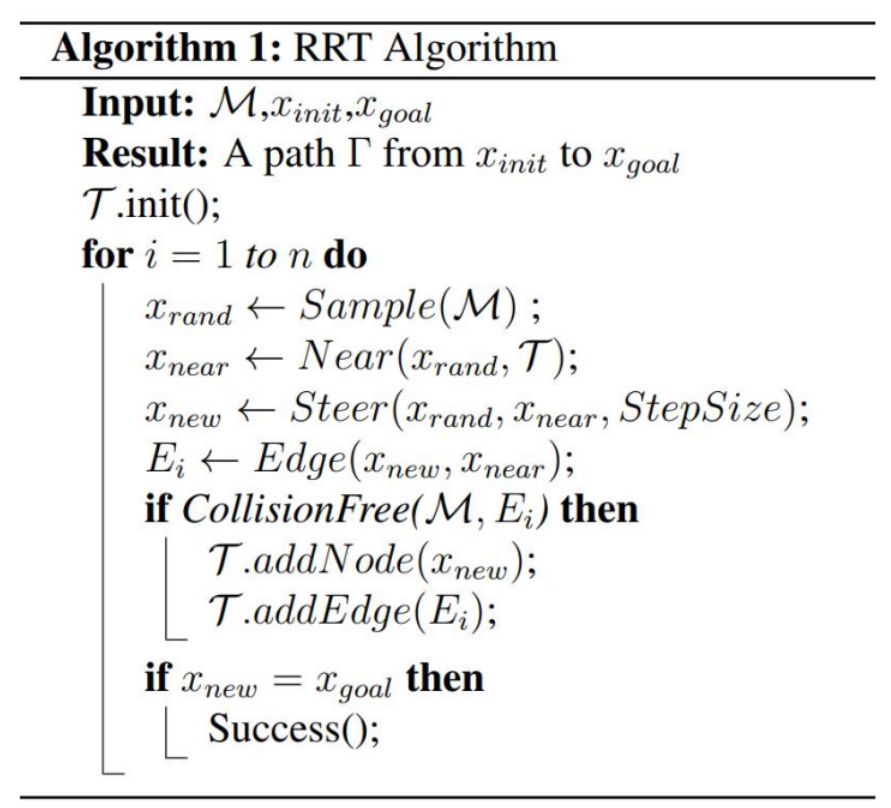
\includegraphics[width=\linewidth]{images/rrt.png}
                \caption{RRT算法流程}
            \end{subfigure}
            \hfill
            \begin{subfigure}[b]{0.50\textwidth}
                \centering
                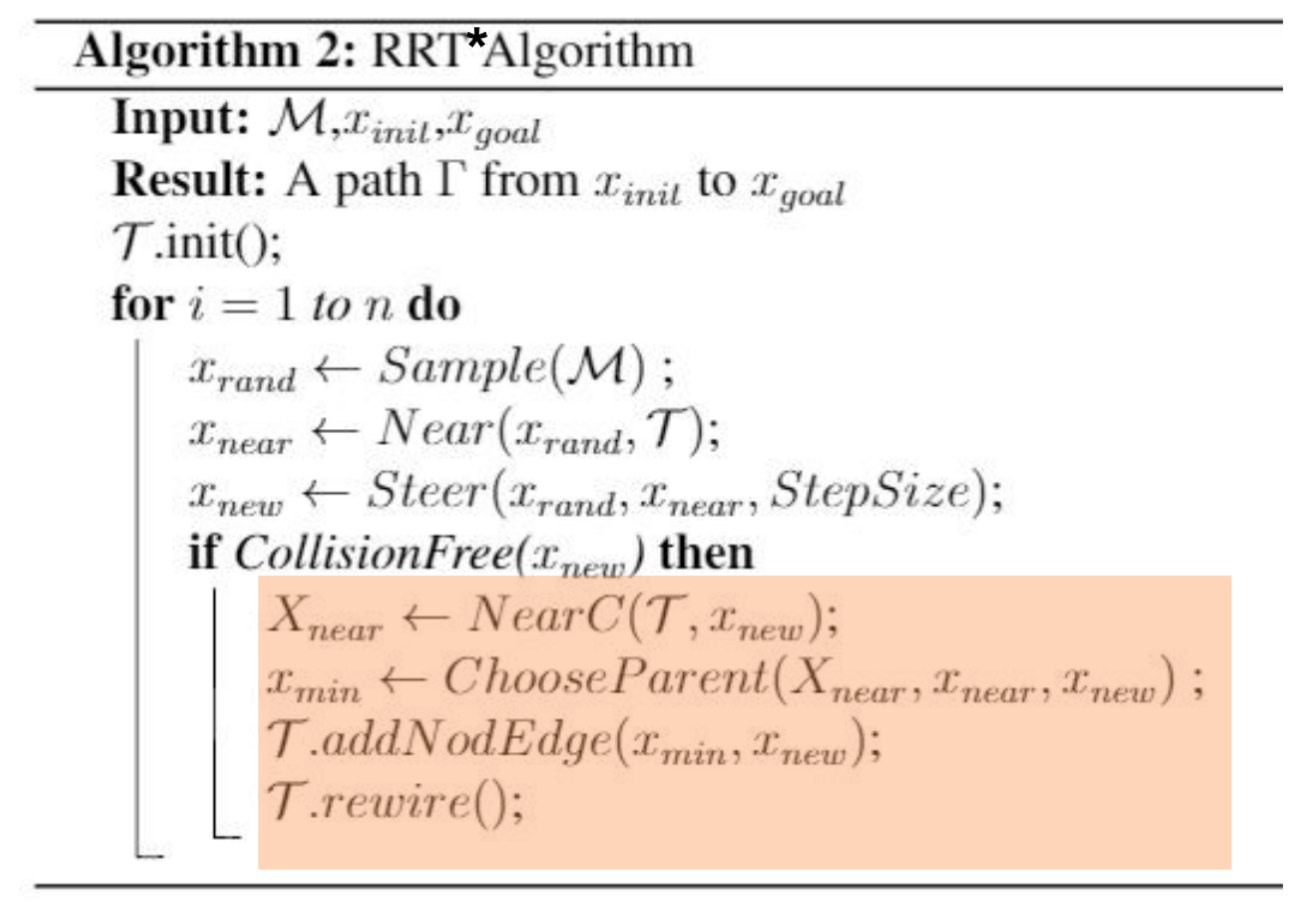
\includegraphics[width=\linewidth]{images/rrts.png}
                \caption{RRT*算法流程}
            \end{subfigure}
        \end{figure}
        \begin{itemize}
            \item \textbf{基本思想}
                \begin{enumerate}
                    \item 连通图采用树的形式,以起始点作为树的根节点
                    \item 采用在空间中随机采样、连接树中最近节点的方式拓展树
                    \item 考虑机器人的运动执行能力
                    \item 通过树结构可以直接回溯得到路径
                \end{enumerate}
            \item \textbf{影响规划收敛速度的三个步骤}
                \begin{itemize}
                    \item sample:随机状态的采样
                    \item near:在搜索树中查找与随机状态距离最近的节点
                    \item collision:新生成节点的防碰检测
                \end{itemize}
        \end{itemize}
        \begin{enumerate}
            \item \textbf{RRT改进算法1}\label{item:prob:rrt:improv1}
                \begin{itemize}
                    \item \textbf{针对问题}:RRT扩张偏向状态空间未探测部分,但不是偏向目标点,当环境复杂时计算效率低
                    \item \textbf{解决办法}:双向搜索Bidirectional-RRT\footnote{使用两棵树(或搜索图)来实现路径规划,分别从起点和终点出发。每次生成两个随机点进行路径生长。一旦两棵树在某处相交,就可以找到一条从起点到终点的路径,因此搜索一定程度上会更加高效。}
                \end{itemize}
            \item \textbf{RRT改进算法2}\label{item:prob:rrt:improv2}
                \begin{itemize}
                    \item \textbf{针对问题}:随机性小步扩展导致路径曲折,成本高

                    \item \textbf{解决办法}:RRT*(加入$h(n)$,实现渐进最优,新节点加入时根据路径成本进行树结构优化)
                        \begin{enumerate}
                            \item 寻找树中新节点邻域内到新节点路径最短的节点,建立连接,加入树集合
                            \item 对树中新节点邻域内节点进行判断,如果从新节点到该节点形成的路径优于现有树中路径,则将该节点父节点修改为新节点
                        \end{enumerate}
                \end{itemize}
        \end{enumerate}
        \begin{figure}[H]
                \centering
                \begin{subfigure}[b]{0.19\textwidth}
                    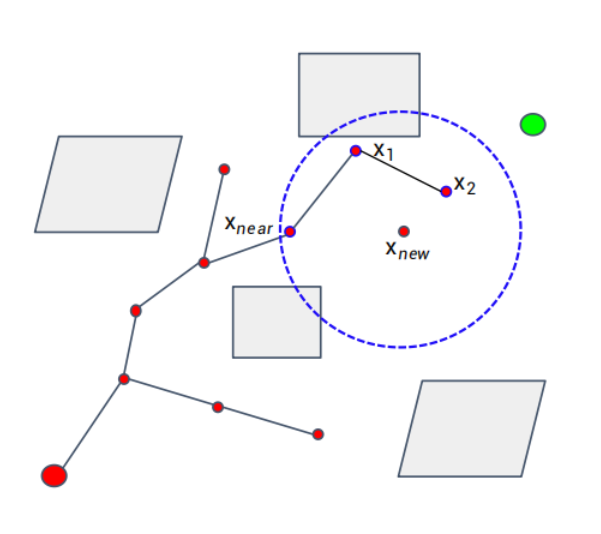
\includegraphics[width=\linewidth]{images/rrts/rrts1.png}
                    \caption{NearC: 选择多个邻节点}
                    \label{fig:rrts1}
                \end{subfigure}
                \begin{subfigure}[b]{0.19\textwidth}
                    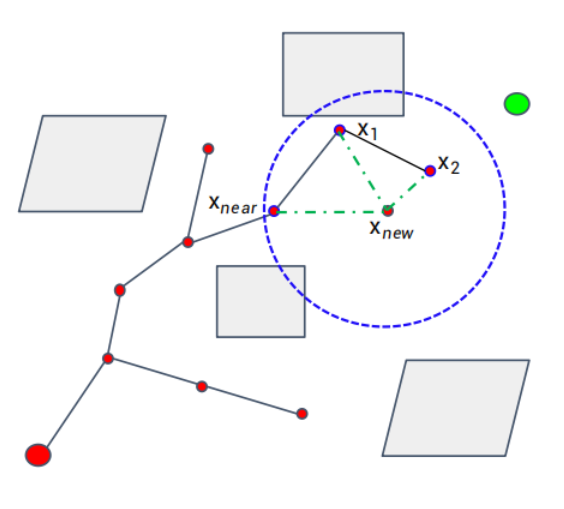
\includegraphics[width=\linewidth]{images/rrts/rrts2.png}
                    \caption{ChooseParent: 评估各邻节点作为父节点下的总路径长度}
                    \label{fig:rrts2}
                \end{subfigure}
                \begin{subfigure}[b]{0.19\textwidth}
                    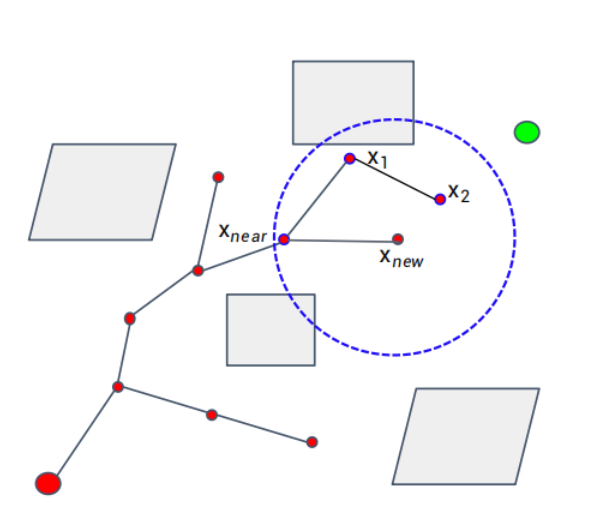
\includegraphics[width=\linewidth]{images/rrts/rrts3.png}
                    \caption{addNodEdge: 根据总最短路径选择父节点}
                    \label{fig:rrts3}
                \end{subfigure}
                \begin{subfigure}[b]{0.19\textwidth}
                    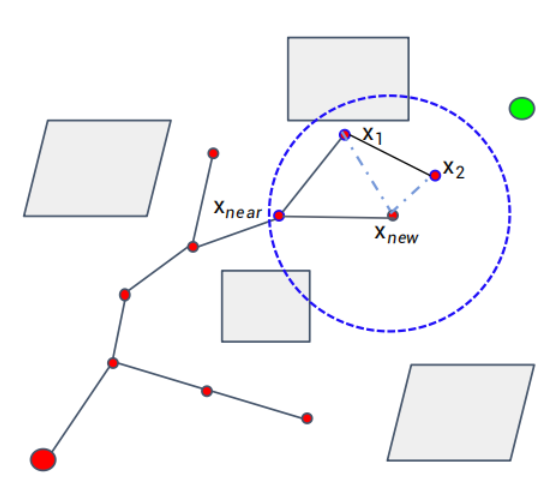
\includegraphics[width=\linewidth]{images/rrts/rrts4.png}
                    \caption{比较最短路径}
                    \label{fig:rrts4}
                \end{subfigure}
                \begin{subfigure}[b]{0.19\textwidth}
                    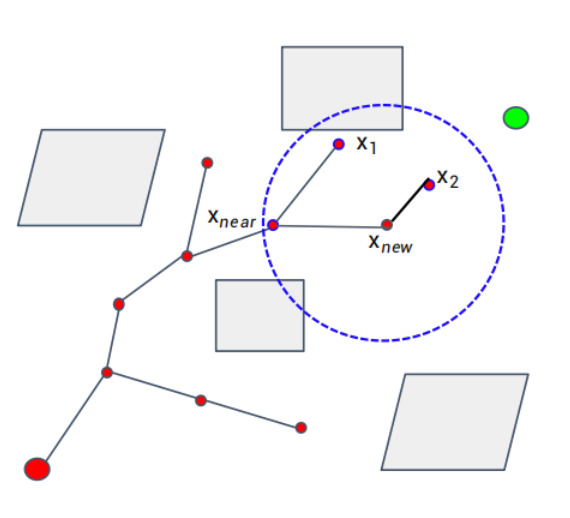
\includegraphics[width=\linewidth]{images/rrts/rrts5.png}
                    \caption{rewrite: 优化邻节点路径(修改父节点)}
                    \label{fig:rrts5}
                \end{subfigure}
                \caption{RRT*算法优化流程可视化}
                \label{fig:rrts_process}
            \end{figure}
    \textcolor{red}{注意:PRM不考虑机器人的执行性,RRT考虑!}
    \end{enumerate}

\subsection{路径规划近期研究}\label{subsec:recent_research}
\begin{itemize}
    \item \textbf{地图形式的优化}\label{item:recent:map}
        \begin{enumerate}
            \item \textbf{ESDF}\label{item:recent:map:esdf}
            \item \textbf{TSDF}\label{item:recent:map:tsdf}
        \end{enumerate}
    \item \textbf{采用学习的方法}\label{item:recent:learning}
        \begin{enumerate}
            \item \textbf{用深度学习学RRT采样分布}\label{item:recent:learning:deep_rrt}
        \end{enumerate}
    \item \textbf{SOCIAL行为路径规划}\label{item:recent:social}
\end{itemize}

\subsection{本章小节}
\begin{table}[H]
    \centering
    \small
    \begin{tabular}{p{4cm}p{5.5cm}p{5.5cm}}
        \toprule
        \textbf{比较维度} & \textbf{分辨率完备方法} & \textbf{概率完备方法} \\
        \midrule
        (1)空间离散采样 & 基于\textbf{解析计算}的姿态空间分解 & 基于\textbf{随机采样}生成连通图或者树 \\
        (2)位形空间连通性表示 & \textbf{完全表达}自由空间的连通性,高维情况下\textbf{计算负担重} & \textbf{近似表达}连通性,但\textbf{计算快速},只需计算单个机器人姿态是否碰撞,其效率与碰撞检测模块效率相关 \\
        \bottomrule
    \end{tabular}
    \caption{分辨率完备与概率完备方法比较}
    \label{tab:resolution_vs_probabilistic}
\end{table}
\end{document}